\documentclass[a4paper,12pt]{article}
\usepackage[T2A]{fontenc}
\usepackage[utf8x]{inputenc}
\usepackage[english,russian]{babel}
\usepackage{amssymb,amsfonts,amsmath,mathtext}
\usepackage[unicode]{hyperref}
\usepackage{listings}
\usepackage{graphicx}
\usepackage{float}
\graphicspath{{images/}}
\newcommand{\anonsection}[1]{\section*{#1}\addcontentsline{toc}{section}{#1}}

\begin{document}

% Титульный лист

\begin{titlepage}
\newpage

\begin{center}

\textit{Министерство науки и высшего образования Российской Федерации \\ 
Федеральное государственное бюджетное образовательное \\
учреждение высшего образования \\
«Московский государственный технический университет \\
имени Н.Э. Баумана (национальный исследовательский университет)» \\
(МГТУ им. Н.Э. Баумана) \\}
\hrulefill
\end{center}

\vspace{2em}

\begin{flushleft}
ФАКУЛЬТЕТ <<Информатика и системы управления>> \\
\vspace{0.5em}
КАФЕДРА <<Программное обеспечение ЭВМ и информационные технологии>>
\end{flushleft}


\vspace{8em}

\begin{center}
\LARGE Рубежный контроль №2 \\
\end{center}

\vspace{1.5em}

\begin{center}
\textsc{Поиск в словаре}
\end{center}

\vspace{6em}

\begin{center}
Головнев Н.В.

\vspace{4em}

ИУ7-54Б
\end{center}

\vspace{\fill}

\begin{center}
Москва 2019
\end{center}

\end{titlepage}

\tableofcontents

% Введение

\newpage

\newpage
\anonsection{ПОСТАНОВКА ЗАДАЧИ}
Найти набольшие участки, совпадающие у двух строк. Сложность поиска подстроки должна быть строго меньше $\theta(n^2)$.

\newpage
\section{АНАЛИТИЧЕСКАЯ ЧАСТЬ}
\subsection{Описание алгоритма}
Пусть $V$ - заданный алфавит, символ $0$ - начало любой строки, <<нулевой символ>>. Тогда словарь можно представить как древовидную структуру (конечный автомат) вида: \\
\begin{figure}[H]
\center{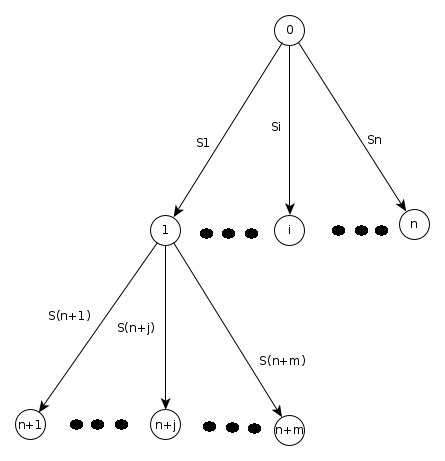
\includegraphics[scale=0.5]{automat1.png}}
\caption{Структура словаря (конечного автомата)}
\label{images:automat1}
\end{figure}

Для того, чтобы найти наибольшие совпадающие участки 2-х строк, можно сделать так:\\
1)Выделить среди строки последовательность строк таким образом, чтобы каждая строка начиналась со 2-ого символа предыдущей строки и заканчивалась последним символом предыдущей. Например: из слова <<abcabdfa>> получим <<abcabdfa>>, <<bcabdfa>>, <<cabdfa>>, ..., <<fa>>, <<a>>.\\
2)Создадим словарь из полученных строк. В результате получим:
\newpage
\begin{figure}[h]
\center{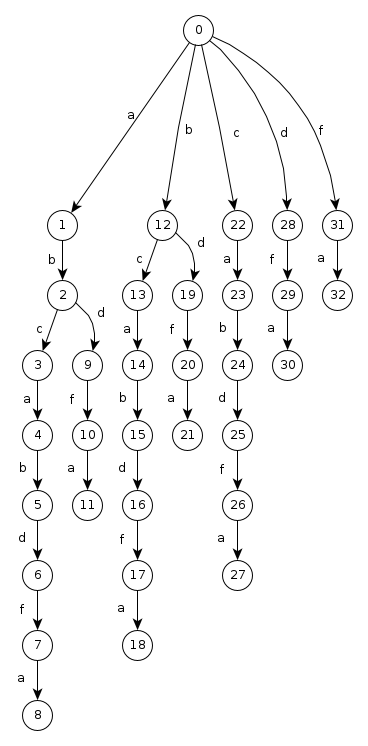
\includegraphics[scale=0.5]{automat2.png}}
\caption{Структура словаря из примера}
\label{images:automat2}
\end{figure} 
3)Превратим его в конечный автомат вида:
\newpage
\begin{figure}[H]
\center{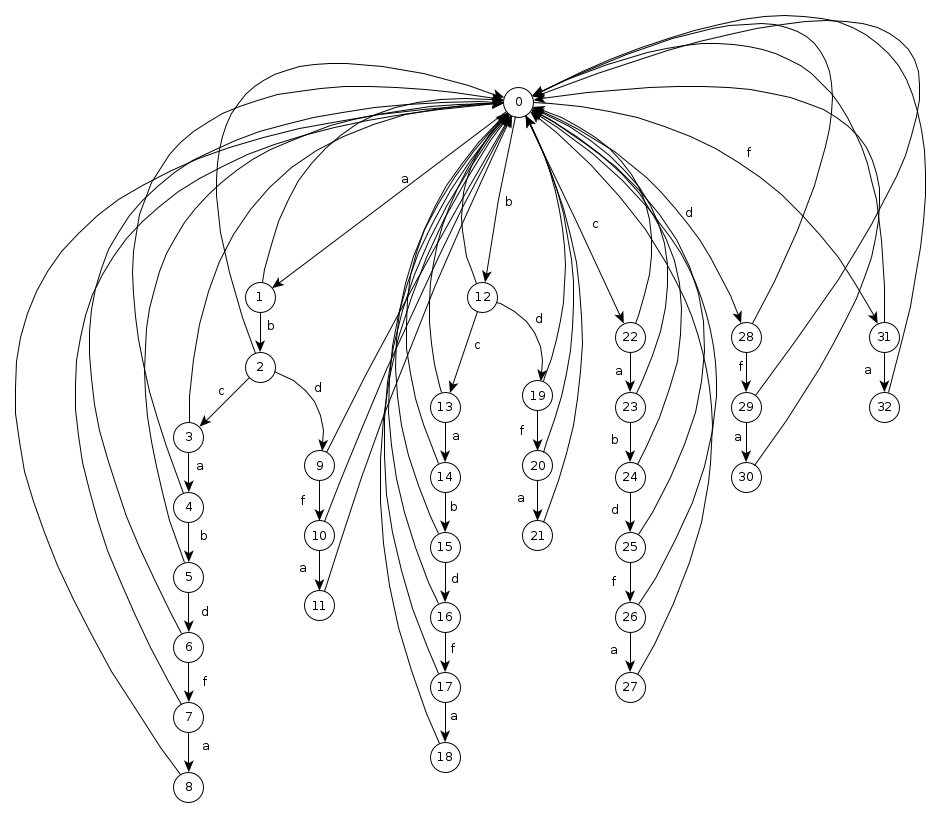
\includegraphics[scale=0.5]{automat3.png}}
\caption{Структура итогового конечного автомата}
\label{images:automat3}
\end{figure}
\newpage
4)Осуществим сам алгоритм поиска, который в случае в попадание в состояние автомата 0 обнуляет текущую длину строки, иначе увеличивает текущую длину строки. Если текущая строка больше максимальной, то сохраняется длина этой подстроки и ее начальная позиция.

\newpage
\section{ТЕХНОЛОГИЧЕСКАЯ ЧАСТЬ}
\subsection{Требования к программному обеспечению}
Программа должна работать на операционной системе Arch Linux. 
Программа должна запускаться из консоли (или терминала) следующей командой:\\
\textit{./app.exe dictionary.txt text.txt} \\
\textit{app.exe} - само приложение. \textit{dictionary.txt} - файл со словами, которые загружаются словарь. На каждой строке должно располагаться одно слово без разделительных знаков. \textit{text.txt} - файл с текстом, в котором ищутся слова, отсутствующие в словаре.
На выход программа должна печатать все слова, не найденные в этом словаре.

\newpage
\subsection{Средства реализации}
Для реализации данных алгоритмов был выбран язык программирования С, компилятор gcc и некоторые функции из библиотеки glibc (memcpy, malloc и тд...). \\
Основные особенности Си: \\
\begin{itemize}
\item простая языковая база, из которой в стандартную библиотеку вынесены многие существенные возможности, вроде математических функций или функций работы с файлами;
\item ориентация на процедурное программирование;
\item использование препроцессора для абстрагирования однотипных операций;
\item доступ к памяти через использование указателей;
\item передача параметров в функцию по значению, а не по ссылке (передача по ссылке эмулируется с помощью указателей);
\item наличие указателей на функции и статических переменных;
\item области видимости имён;
\item структуры и объединения — определяемые пользователем собирательные типы данных, которыми можно манипулировать как одним целым.
\end{itemize}


\newpage
\subsection{Листинг кода}
Ниже приведена реализация алгоритма на С.\\
\lstdefinestyle{customc}{
  belowcaptionskip=1\baselineskip,
  breaklines=true,
  frame=L,
  xleftmargin=\parindent,
  language=C,
  showstringspaces=false,
  basicstyle=\footnotesize\ttfamily
}
\lstinputlisting[captionpos=b, caption=\label{listings:listing1}Реализация алгоритма поиска в словаре(\ref{images:scheme1}), style=customc]{listing1.c}
\lstinputlisting[captionpos=b, caption=\label{listings:listing2}Структура узла дерева, style=customc]{listing2.c}

\newpage
\section{ЭКСПЕРИМЕНТАЛЬНАЯ ЧАСТЬ}
\subsection{Характеристики аппаратного и программного обеспечения}
% Часть которую никогда нельзя менять
Тестирование приложения проводилось на машине со следующими характеристиками:\\
\begin{itemize}
\item Процессор Intel® Core™ i7-7700HQ;
\item Оперативная память 16 ГБ;
\item Операционная система - Arch Linux с рабочим окружением Cinnamon.
\end{itemize}

\newpage
\subsection{Примеры работы}
На рис. \ref{images:example}, предсавленном ниже, демонстрируется работа приложения. Запуск приложения осуществляется из эмулятора терминала в Arch Linux.
\textit{dictionary.txt} - файл, содержащий словарь (каждое слово на отдельной строке).\textit{text.txt} - файл, содержащий текст, в котором происходит поиск слов, отсутствующих в словаре и выводе их на экран. Содержание файла представлено на рис. \ref{images:example1}.
\begin{figure}[h]
\center{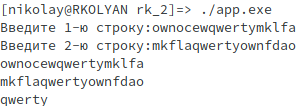
\includegraphics[scale=0.5]{example.png}}
\caption{Пример работы приложения}
\label{images:example}
\end{figure}

\end{document}
